\chapter{Experiments}
\label{chapter:experiments}

\begin{figure}[!tbp]%
	\centering
	\begin{subfigure}[t]{\textwidth}
		\begin{subfigure}[t]{0.45\textwidth}
			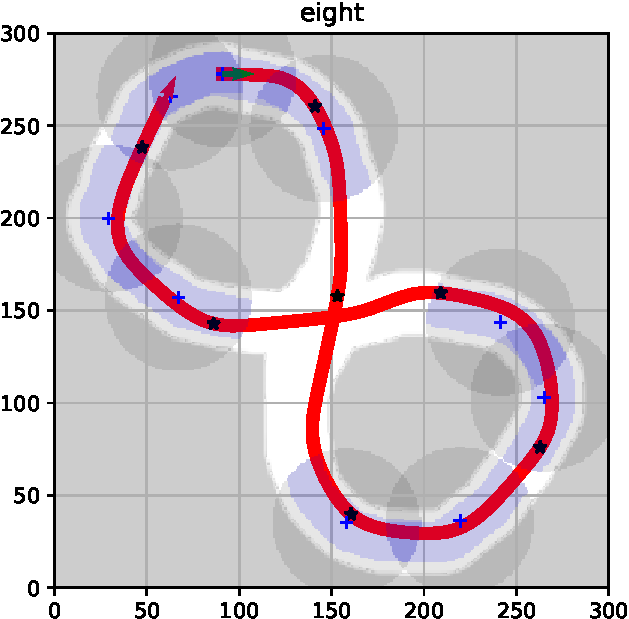
\includegraphics[width=\textwidth]{../img/experiments/eight-hybrid_astar-trajectory}
		\end{subfigure}
		\hfill
		\begin{subfigure}[t]{0.45\textwidth}
			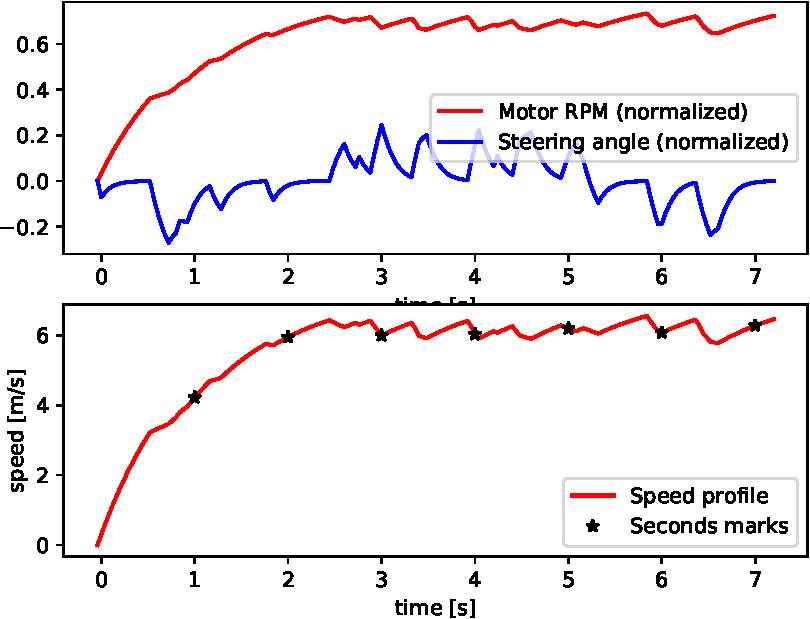
\includegraphics[width=\textwidth]{../img/experiments/eight-hybrid_astar-actuators}
		\end{subfigure}
		\caption{Solution found by Hybrid A*}
		\label{fig:eight-hybrid_astar}
	\end{subfigure}
	
	\vspace{0.75cm}
	
	\begin{subfigure}[t]{\textwidth}
		\begin{subfigure}[t]{0.45\textwidth}
			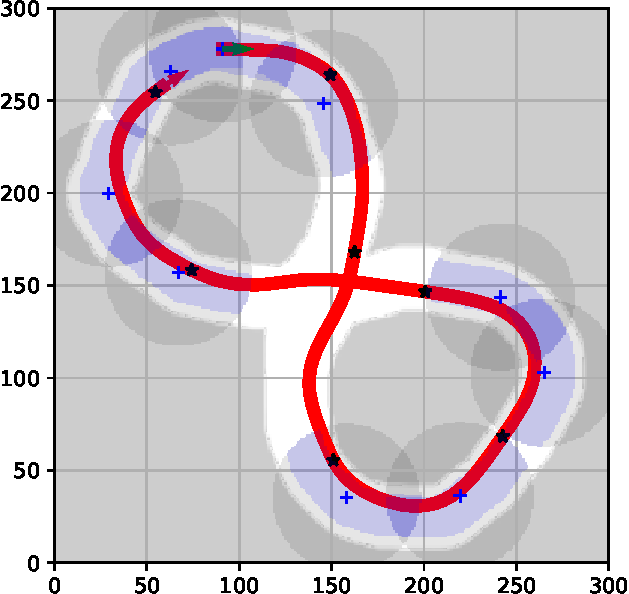
\includegraphics[width=\textwidth]{../img/experiments/eight-sehs-trajectory}
		\end{subfigure}
		\hfill
		\begin{subfigure}[t]{0.45\textwidth}
			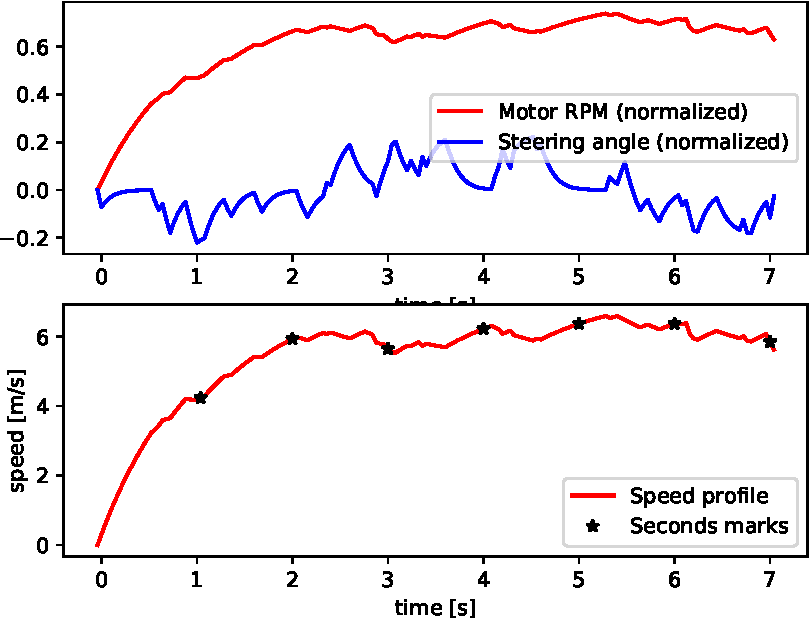
\includegraphics[width=\textwidth]{../img/experiments/eight-sehs-actuators}
		\end{subfigure}
		\caption{Solution found by SEHS}
		\label{fig:eight-sehs}
	\end{subfigure}

	\vspace{0.75cm}

	\begin{subfigure}[t]{\textwidth}
		\centering
		\begin{tabular}{l r r r r r}%
			\toprule
			Algorithm & Opened & Expanded & Search time & Distance & Lap time \\
			\midrule
			Hybrid A* & \textbf{\num{188160}} & \textbf{\num{22173}} & \textbf{\SI{328.57}{\milli\second}} & \SI{40.26}{\meter} & \SI{7.24}{\second} \\
			SEHS & \num{298325} & \num{36008} & \SI{563.19}{\milli\second} & \textbf{\SI{37.77}{\meter}} & \textbf{\SI{6.88}{\second}} \\
			\bottomrule
		\end{tabular}
		\caption{Comparison of the solutions and computation requirements.}
		\label{table:eight}
	\end{subfigure}

	\vspace{0.75cm}

	\caption{Track ``Eight''}
\end{figure}


\begin{figure}[!tbp]%
	\centering

	\begin{subfigure}[t]{\textwidth}
		\begin{subfigure}[t]{0.45\textwidth}
			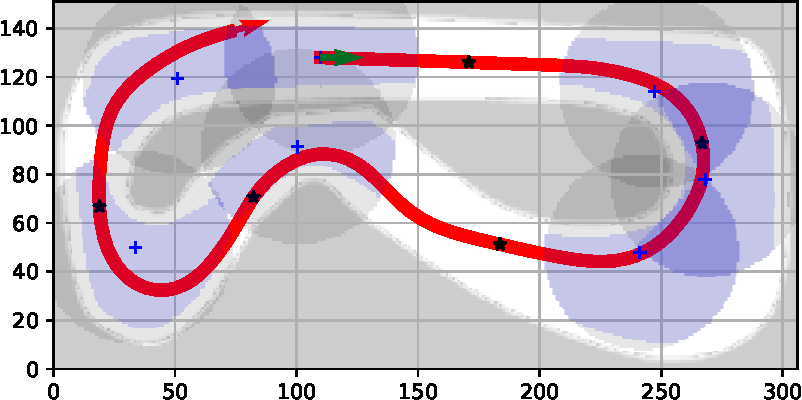
\includegraphics[width=\textwidth]{../img/experiments/porto-hybrid_astar-trajectory}
		\end{subfigure}
		\hfill
		\begin{subfigure}[t]{0.45\textwidth}
			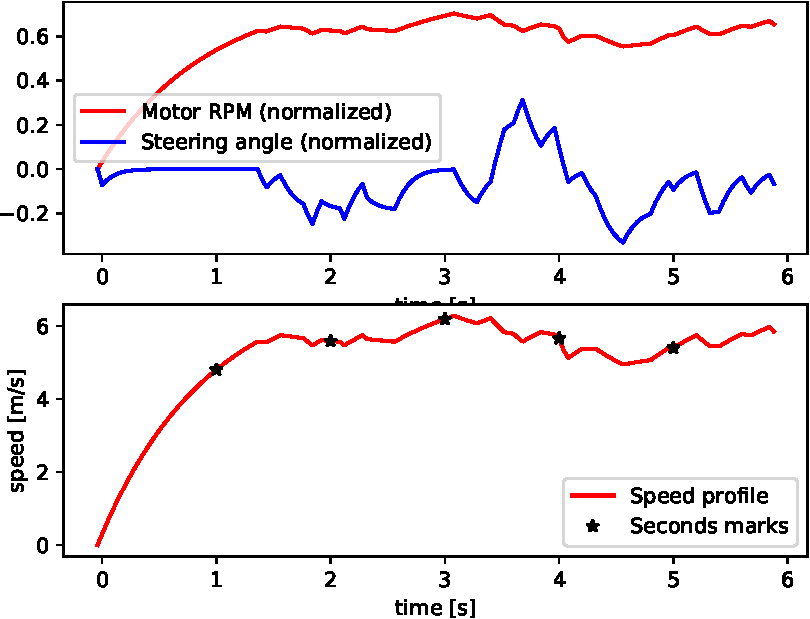
\includegraphics[width=\textwidth]{../img/experiments/porto-hybrid_astar-actuators}
		\end{subfigure}
		\caption{Solution found by Hybrid A*}
		\label{fig:solution_porto-hybrid_astar}	
	\end{subfigure}
	
	\vspace{0.75cm}
	
	\begin{subfigure}[t]{\textwidth}
		\begin{subfigure}[t]{0.45\textwidth}
			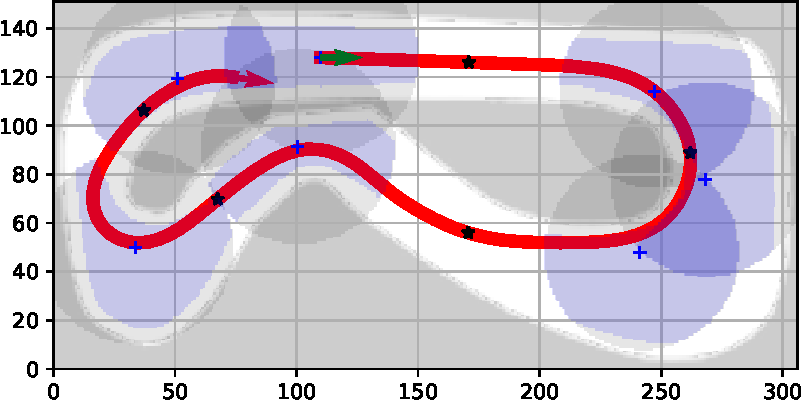
\includegraphics[width=\textwidth]{../img/experiments/porto-sehs-trajectory}
		\end{subfigure}
		\hfill
		\begin{subfigure}[t]{0.45\textwidth}
			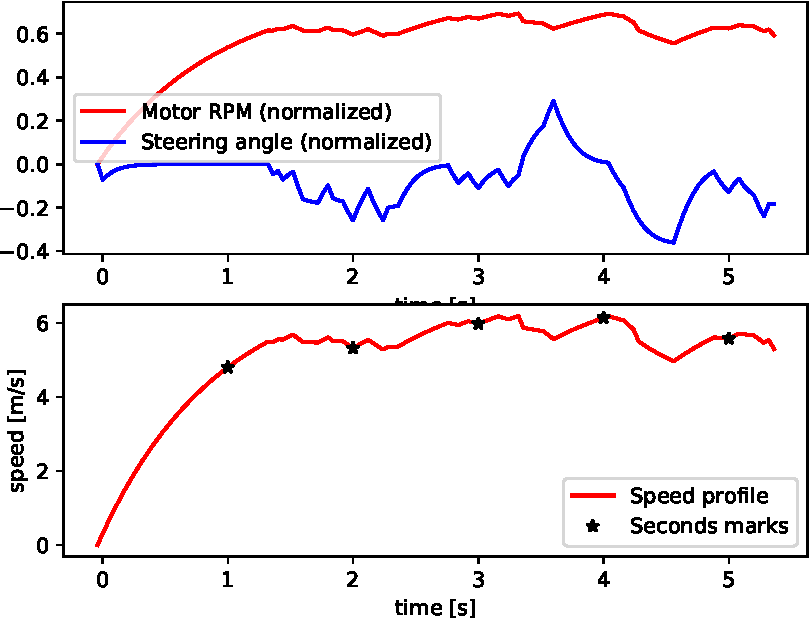
\includegraphics[width=\textwidth]{../img/experiments/porto-sehs-actuators}
		\end{subfigure}
		\caption{Solution found by SEHS}
		\label{fig:solution_porto-sehs}
	\end{subfigure}

	\vspace{0.75cm}
	
	\begin{subfigure}[t]{\textwidth}
		\centering
		\begin{tabular}{l r r r r r}%
			\toprule
			Algorithm & Opened & Expanded & Search time & Distance & Lap time \\
			\midrule
			Hybrid A* & \num{102430} & \num{11957} & \SI{166.55}{\milli\second} & \SI{30.39}{\meter} & \SI{5.92}{\second} \\
			SEHS & \num{93936} & \num{11070} & \SI{165.30}{\milli\second} & \SI{26.88}{\meter} & \SI{5.40}{\second} \\
			\bottomrule
		\end{tabular}
		\caption{Comparison of the solutions and computation requirements.}
		\label{table:porto}
	\end{subfigure}

	\vspace{0.75cm}
	
	\caption{Track ``Porto''}
\end{figure}


\begin{figure}[!tbp]%
	\centering
	
	\begin{subfigure}[t]{\textwidth}
		\begin{subfigure}[t]{0.45\textwidth}
			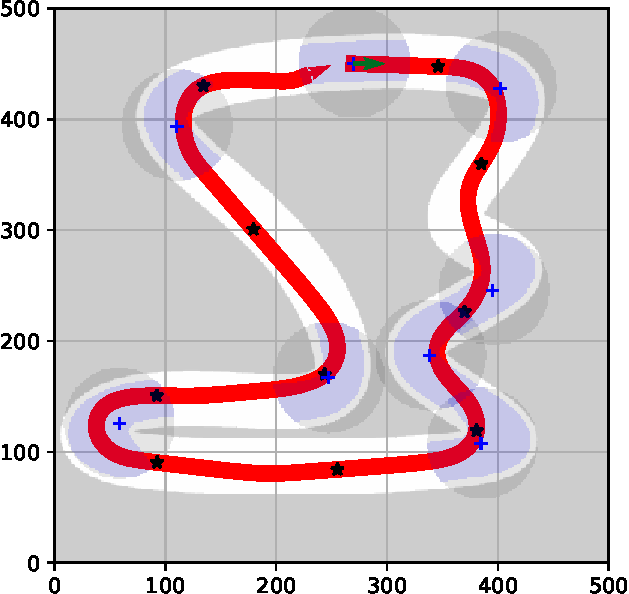
\includegraphics[width=\textwidth]{../img/experiments/tornado-hybrid_astar-trajectory}
		\end{subfigure}
		\hfill
		\begin{subfigure}[t]{0.45\textwidth}
			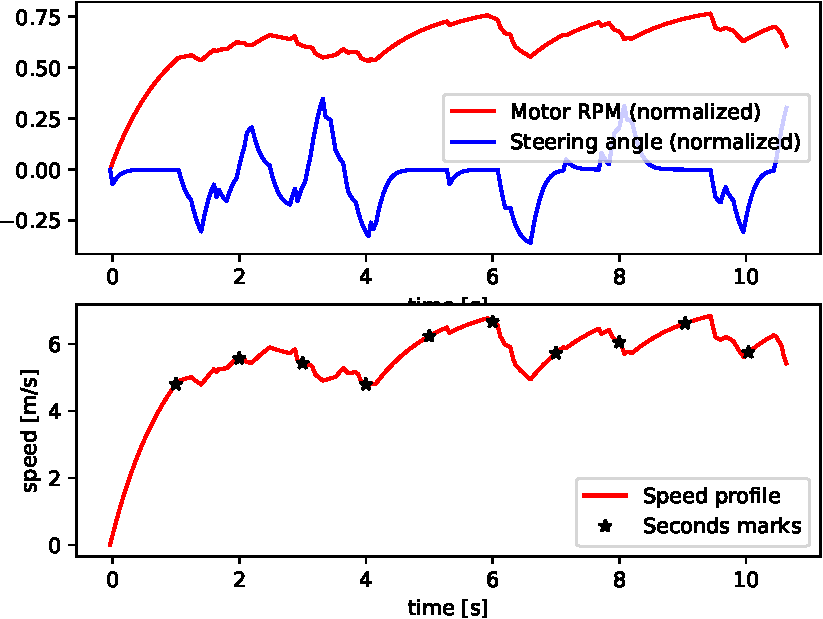
\includegraphics[width=\textwidth]{../img/experiments/tornado-hybrid_astar-actuators}
		\end{subfigure}
		\caption{Solution found by Hybrid A*}
		\label{fig:solution_tornado-hybrid_astar}	
	\end{subfigure}
	
	\vspace{0.75cm}
	
	\begin{subfigure}[t]{\textwidth}
		\begin{subfigure}[t]{0.45\textwidth}
			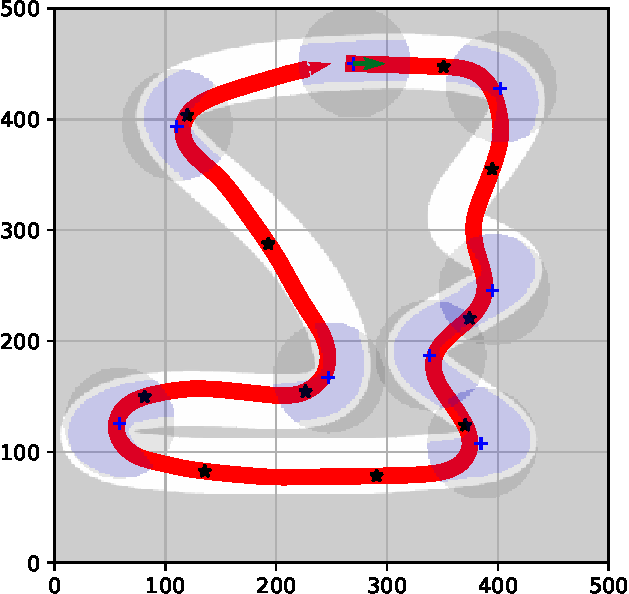
\includegraphics[width=\textwidth]{../img/experiments/tornado-sehs-trajectory}
		\end{subfigure}
		\hfill
		\begin{subfigure}[t]{0.45\textwidth}
			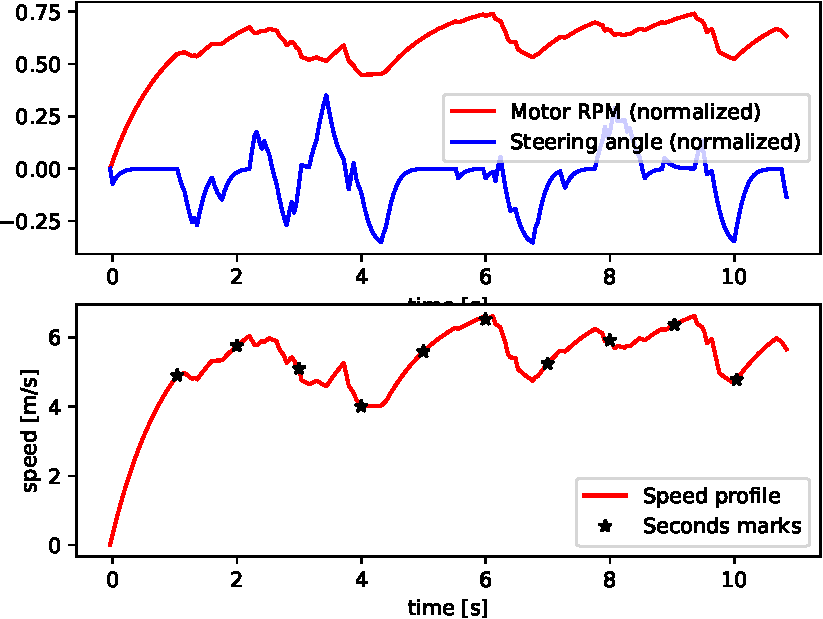
\includegraphics[width=\textwidth]{../img/experiments/tornado-sehs-actuators}
		\end{subfigure}
		\caption{Solution found by SEHS}
		\label{fig:solution_tornado-sehs}
	\end{subfigure}
	
	\vspace{0.75cm}
	
	\begin{subfigure}[t]{\textwidth}
		\centering
		\begin{tabular}{l r r r r r}%
			\toprule
			Algorithm & Opened & Expanded & Search time & Distance & Lap time \\
			\midrule
			Hybrid A* & \num{184864} & \num{21874} & \SI{322.95}{\milli\second} & \SI{59.0759}{\meter} & \SI{10.68}{\second} \\
			SEHS & \num{129022} & \num{15232} & \SI{257.95}{\milli\second} & \SI{57.7269}{\meter} & \SI{10.80}{\second} \\
			\bottomrule
		\end{tabular}
		\caption{Comparison of the solutions and computation requirements.}
		\label{table:tornado}
	\end{subfigure}
	
	\vspace{0.75cm}
	
	\caption{Track ``Tornado''}
\end{figure}

\begin{figure}[!tbp]%
	\centering

	\begin{subfigure}[t]{\textwidth}
		\begin{subfigure}[t]{0.45\textwidth}
			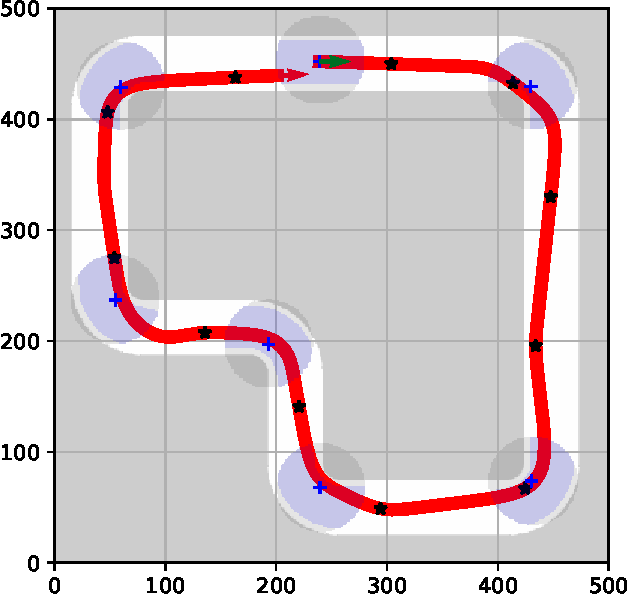
\includegraphics[width=\textwidth]{../img/experiments/simple-hybrid_astar-trajectory}
		\end{subfigure}
		\hfill
		\begin{subfigure}[t]{0.45\textwidth}
			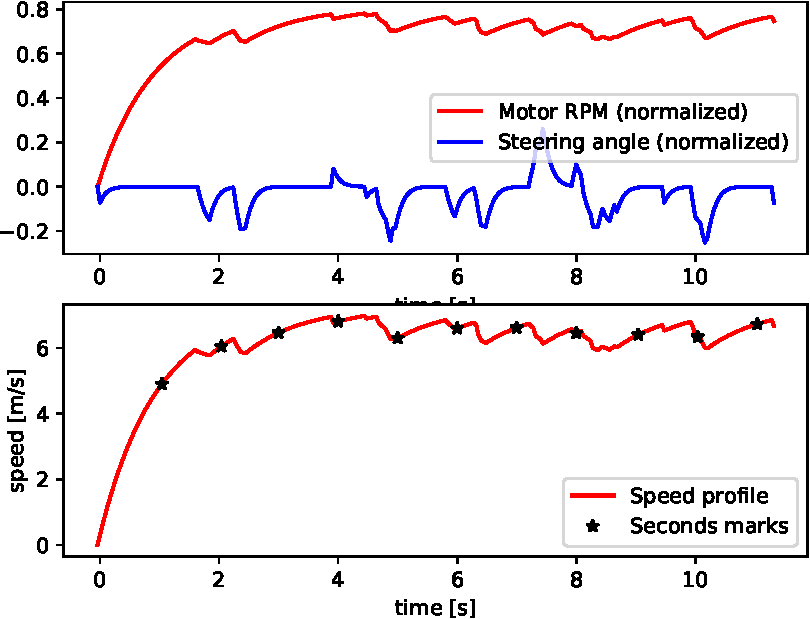
\includegraphics[width=\textwidth]{../img/experiments/simple-hybrid_astar-actuators}
		\end{subfigure}
		\caption{Solution found by Hybrid A*}
		\label{fig:simple-hybrid_astar}
	\end{subfigure}

	\vspace{0.75cm}
	
	\begin{subfigure}[t]{\textwidth}
		\begin{subfigure}[t]{0.45\textwidth}
			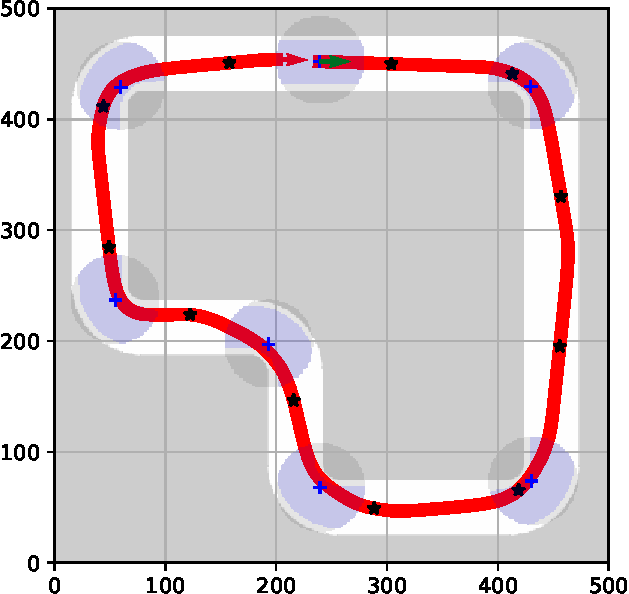
\includegraphics[width=\textwidth]{../img/experiments/simple-sehs-trajectory}
		\end{subfigure}
		\hfill
		\begin{subfigure}[t]{0.45\textwidth}
			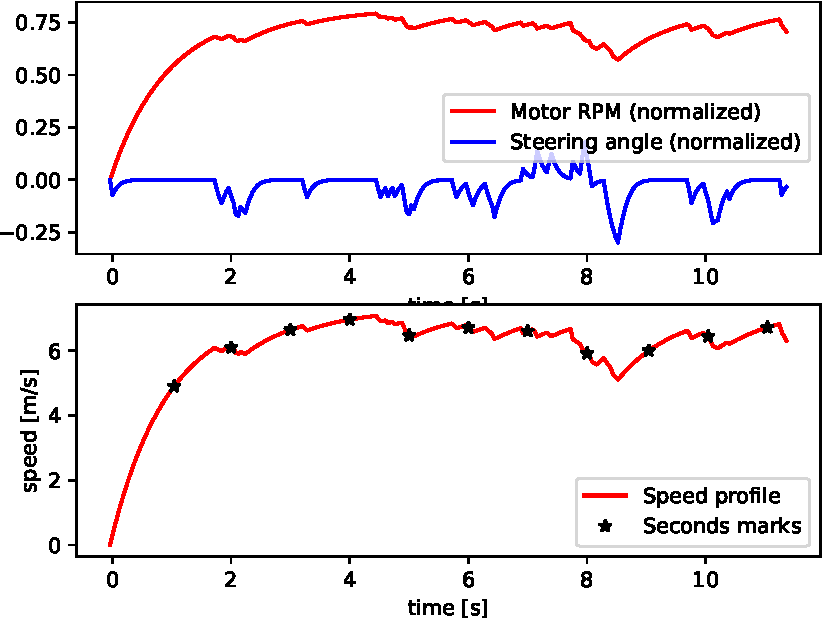
\includegraphics[width=\textwidth]{../img/experiments/simple-sehs-actuators}
		\end{subfigure}
		\caption{Soultion found by SEHS}
		\label{fig:simple-sehs}
	\end{subfigure}

	\vspace{0.75cm}

	\begin{subfigure}[t]{\textwidth}
		\centering
		\begin{tabular}{l r r r r r}%
			\toprule
			Algorithm & Opened & Expanded & Search time & Distance & Lap time \\
			\midrule
			Hybrid A* & \num{324109} & \num{37123} & \SI{549.33}{\milli\second} & \SI{69.18}{\meter} & \SI{11.36}{\second} \\
			SEHS & \num{193095} & \num{22003} & \SI{372.49}{\milli\second} & \SI{69.60}{\meter} & \SI{11.36}{\second} \\
			\bottomrule
		\end{tabular}
		\caption{Comparison of the solutions and computation requirements.}
		\label{table:simple}
	\end{subfigure}
	
	\vspace{0.75cm}

	\caption{Track ``Simple''}
\end{figure}

\begin{figure}[!tbp]%
	\centering

	\begin{subfigure}[t]{\textwidth}
		\begin{subfigure}[t]{0.45\textwidth}
			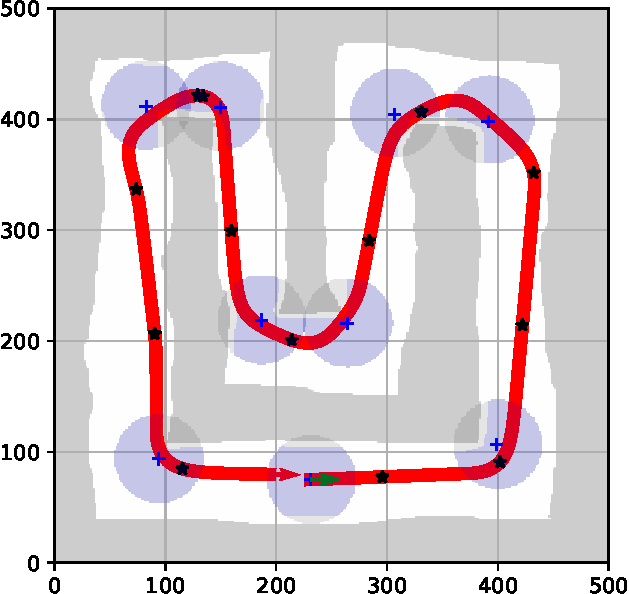
\includegraphics[width=\textwidth]{../img/experiments/u-hybrid_astar-trajectory}
		\end{subfigure}
		\hfill
		\begin{subfigure}[t]{0.45\textwidth}
			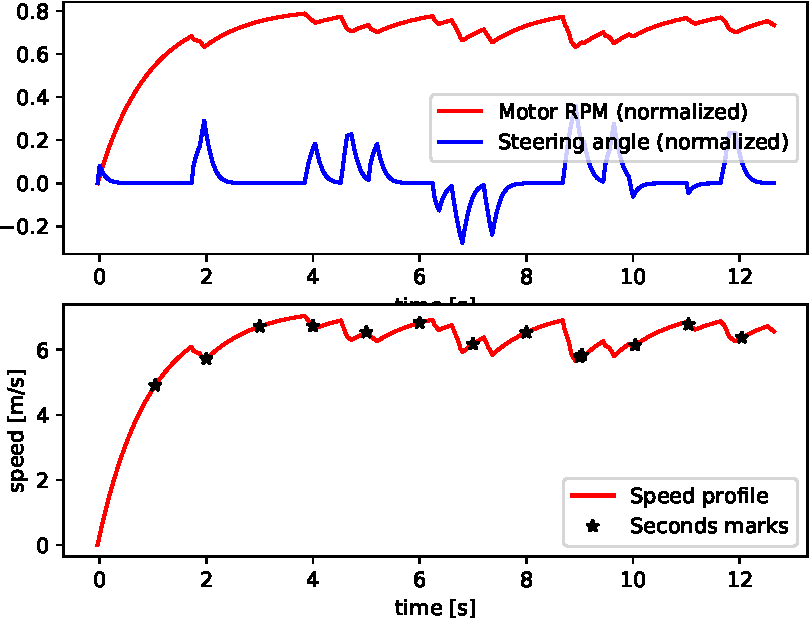
\includegraphics[width=\textwidth]{../img/experiments/u-hybrid_astar-actuators}
		\end{subfigure}	
		\caption{Solution found by Hybrid A*}
		\label{fig:u-hybrid_astar}
	\end{subfigure}

	\vspace{0.75cm}

	\begin{subfigure}[t]{\textwidth}
		\begin{subfigure}[t]{0.45\textwidth}
			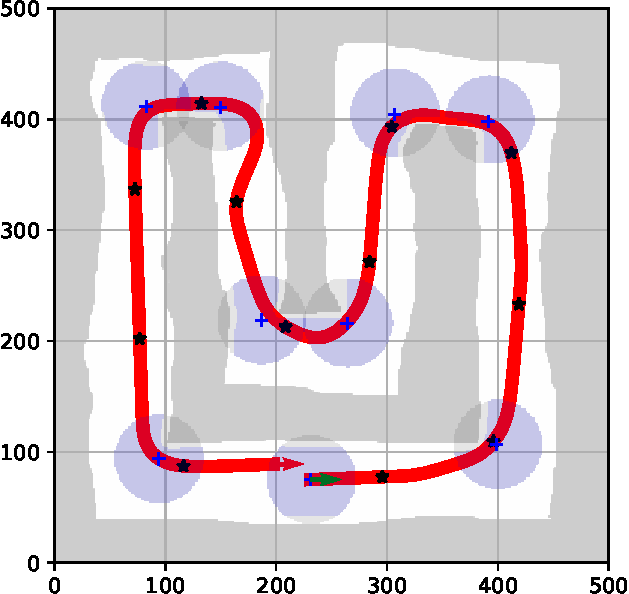
\includegraphics[width=\textwidth]{../img/experiments/u-sehs-trajectory}
		\end{subfigure}
		\hfill
		\begin{subfigure}[t]{0.45\textwidth}
			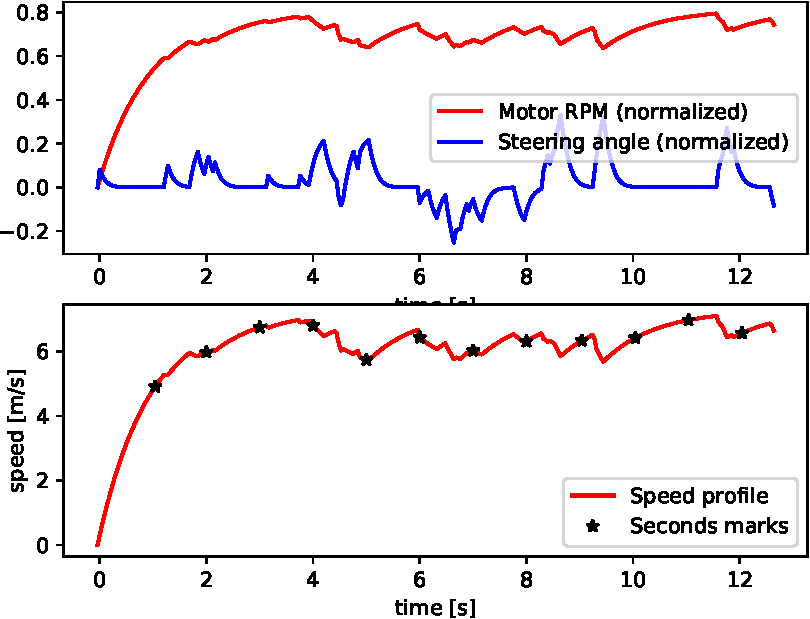
\includegraphics[width=\textwidth]{../img/experiments/u-sehs-actuators}
		\end{subfigure}
		\caption{Solution found by SEHS}
		\label{fig:u-sehs}
	\end{subfigure}
	
	\vspace{0.75cm}
	
	\begin{subfigure}[t]{\textwidth}
		\centering
		\begin{tabular}{l r r r r r}%
		\toprule
		Algorithm & Opened & Expanded & Search time & Distance & Lap time \\
		\midrule
		Hybrid A* & \num{20297799} & \num{2472203} & \SI{64290.3}{\milli\second} & \SI{77.79}{\meter} & \SI{12.68}{\second} \\
		SEHS & \num{4949842} & \num{590288} & \SI{14058.7}{\milli\second} & \SI{75.91}{\meter} & \SI{12.56}{\second} \\
		\bottomrule
	\end{tabular}
	\caption{Comparison of the solutions and computation requirements.}
	\label{table:u}
	\end{subfigure}
	
	\vspace{0.75cm}
	
	\caption{Track ``U''}
\end{figure}

\begin{figure}[!tbp]%
	\centering
		
	\begin{subfigure}[t]{\textwidth}
		\begin{subfigure}[t]{0.45\textwidth}
			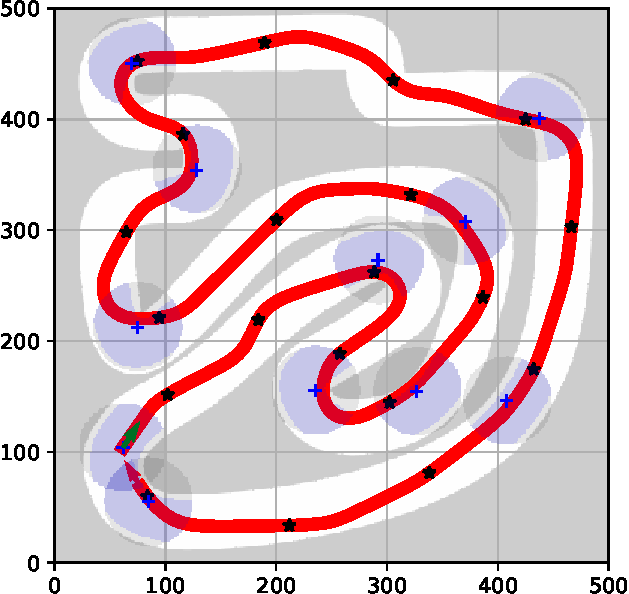
\includegraphics[width=\textwidth]{../img/experiments/zurich-hybrid_astar-trajectory}
		\end{subfigure}
		\hfill
		\begin{subfigure}[t]{0.45\textwidth}
			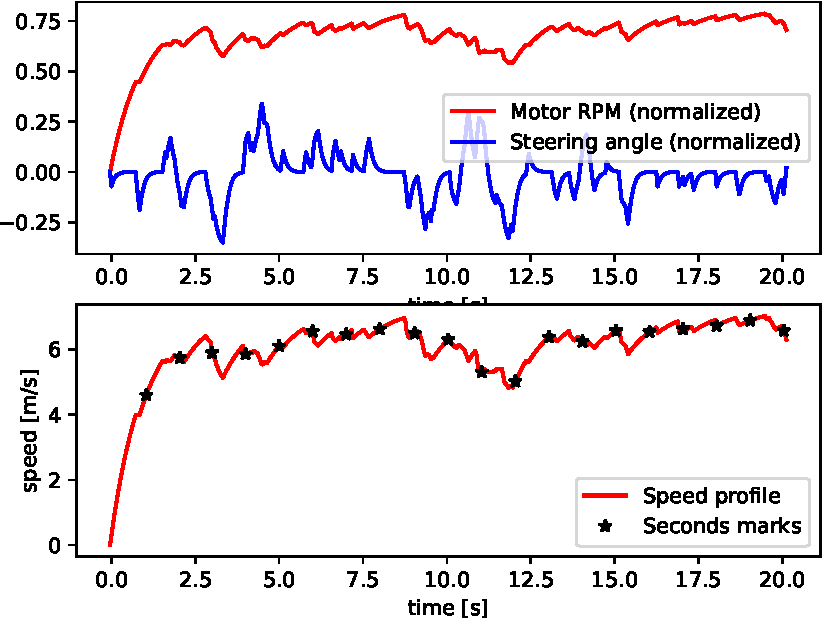
\includegraphics[width=\textwidth]{../img/experiments/zurich-hybrid_astar-actuators}
		\end{subfigure}
		\caption{Solution found by Hybrid A*}
		\label{fig:zurich-hybrid_astar}
	\end{subfigure}

	\vspace{0.75cm}
	
	\begin{subfigure}[t]{\textwidth}	
		\begin{subfigure}[t]{0.45\textwidth}
			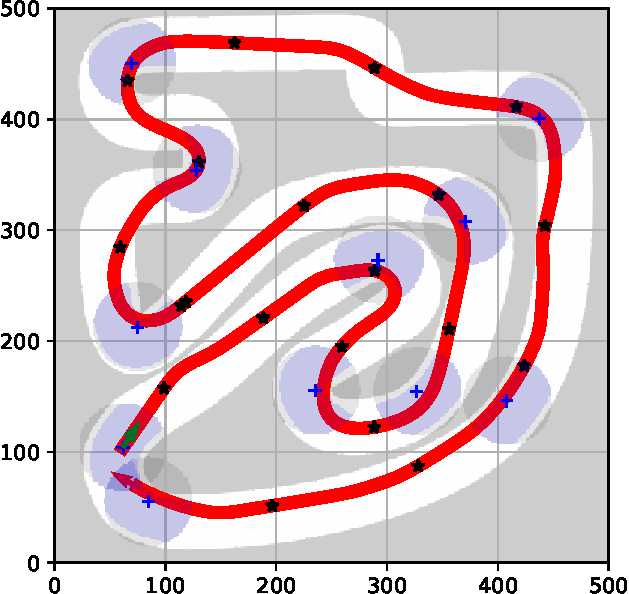
\includegraphics[width=\textwidth]{../img/experiments/zurich-sehs-trajectory}
		\end{subfigure}
		\hfill
		\begin{subfigure}[t]{0.45\textwidth}
			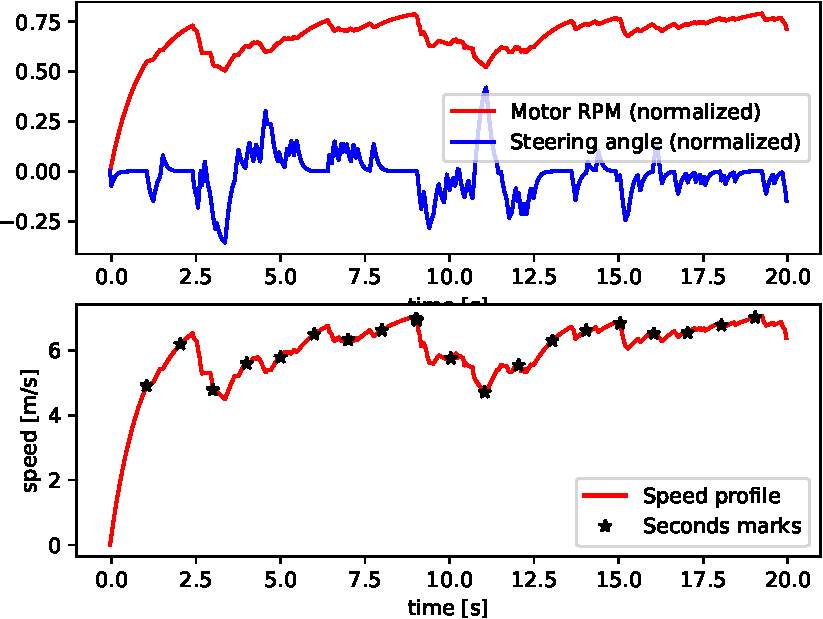
\includegraphics[width=\textwidth]{../img/experiments/zurich-sehs-actuators}
		\end{subfigure}
		\caption{Solution found by SEHS}
		\label{fig:zurich-sehs}
	\end{subfigure}

	\vspace{0.75cm}
	
	\begin{subfigure}[t]{\textwidth}
		\centering
		\begin{tabular}{l r r r r r}%
			\toprule
			Algorithm & Opened & Expanded & Search time & Distance & Lap time \\
			\midrule
			Hybrid A* & \num{5934391} & \num{715557} & \SI{13579.90}{\milli\second} & \SI{121.58}{\meter} & \SI{20.16}{\second} \\
			SEHS & \num{1585340} & \num{590288} & \SI{4078.63}{\milli\second} & \SI{121.61}{\meter} & \SI{20.32}{\second} \\
			\bottomrule
		\end{tabular}
		\caption{Comparison of the solutions and computation requirements.}
		\label{table:zurich}
	\end{subfigure}
	
	\vspace{0.75cm}

	\caption{Track ``Zurich''}
\end{figure}